%% LaTeX-Beamer template for KIT design
%% by Erik Burger, Christian Hammer
%% title picture by Klaus Krogmann
%%
%% version 2.1
%%
%% mostly compatible to KIT corporate design v2.0
%% http://intranet.kit.edu/gestaltungsrichtlinien.php
%%
%% Problems, bugs and comments to
%% burger@kit.edu

\documentclass[18pt]{beamer}

%% SLIDE FORMAT

% use 'beamerthemekit' for standard 4:3 ratio
% for widescreen slides (16:9), use 'beamerthemekitwide'

\usepackage{templates/beamerthemekit}
% \usepackage{templates/beamerthemekitwide}

%% TITLE PICTURE

% if a custom picture is to be used on the title page, copy it into the 'logos'
% directory, in the line below, replace 'mypicture' with the 
% filename (without extension) and uncomment the following line
% (picture proportions: 63 : 20 for standard, 169 : 40 for wide
% *.eps format if you use latex+dvips+ps2pdf, 
% *.jpg/*.png/*.pdf if you use pdflatex)

%\titleimage{mypicture}

%% TITLE LOGO

% for a custom logo on the front page, copy your file into the 'logos'
% directory, insert the filename in the line below and uncomment it

\titlelogo{empty}

% (*.eps format if you use latex+dvips+ps2pdf,
% *.jpg/*.png/*.pdf if you use pdflatex)

%% TikZ INTEGRATION

% use these packages for PCM symbols and UML classes
\usepackage{templates/tikzkit}
\usepackage{templates/tikzuml}

% the presentation starts here

\title[Snow Scene]{Freestyle Assginment:\\ Snow Scene}
\subtitle{For Graphikprogrammierung und Anwendung WS 2018}
\author{Julian Spittel}

\institute{Computer Graphics Group}

% Bibliography

\usepackage[citestyle=authoryear,bibstyle=numeric,hyperref,backend=biber]{biblatex}
\addbibresource{templates/example.bib}
\bibhang1em

\begin{document}

% change the following line to "ngerman" for German style date and logos
\selectlanguage{english}

%title page
\begin{frame}
\titlepage
\end{frame}

\section{Introduction}
\begin{frame}{The Concept}
A snowy scenery that includes:
\begin{itemize}
\item A snowfall particle system
\item Volumetric snow on top of the terrain
\item A system that tracks footprints
\item Snowfall that increases the amount of volumetric snow and refills footprints
\item Snow height and refill rates depending on terrain(slope, height)
\item Snowy trees
\end{itemize}
\end{frame}

\section{Implementation}


\subsection{Particle System}
\begin{frame}{Particle System}
	\begin{figure}[H]
		\centering
		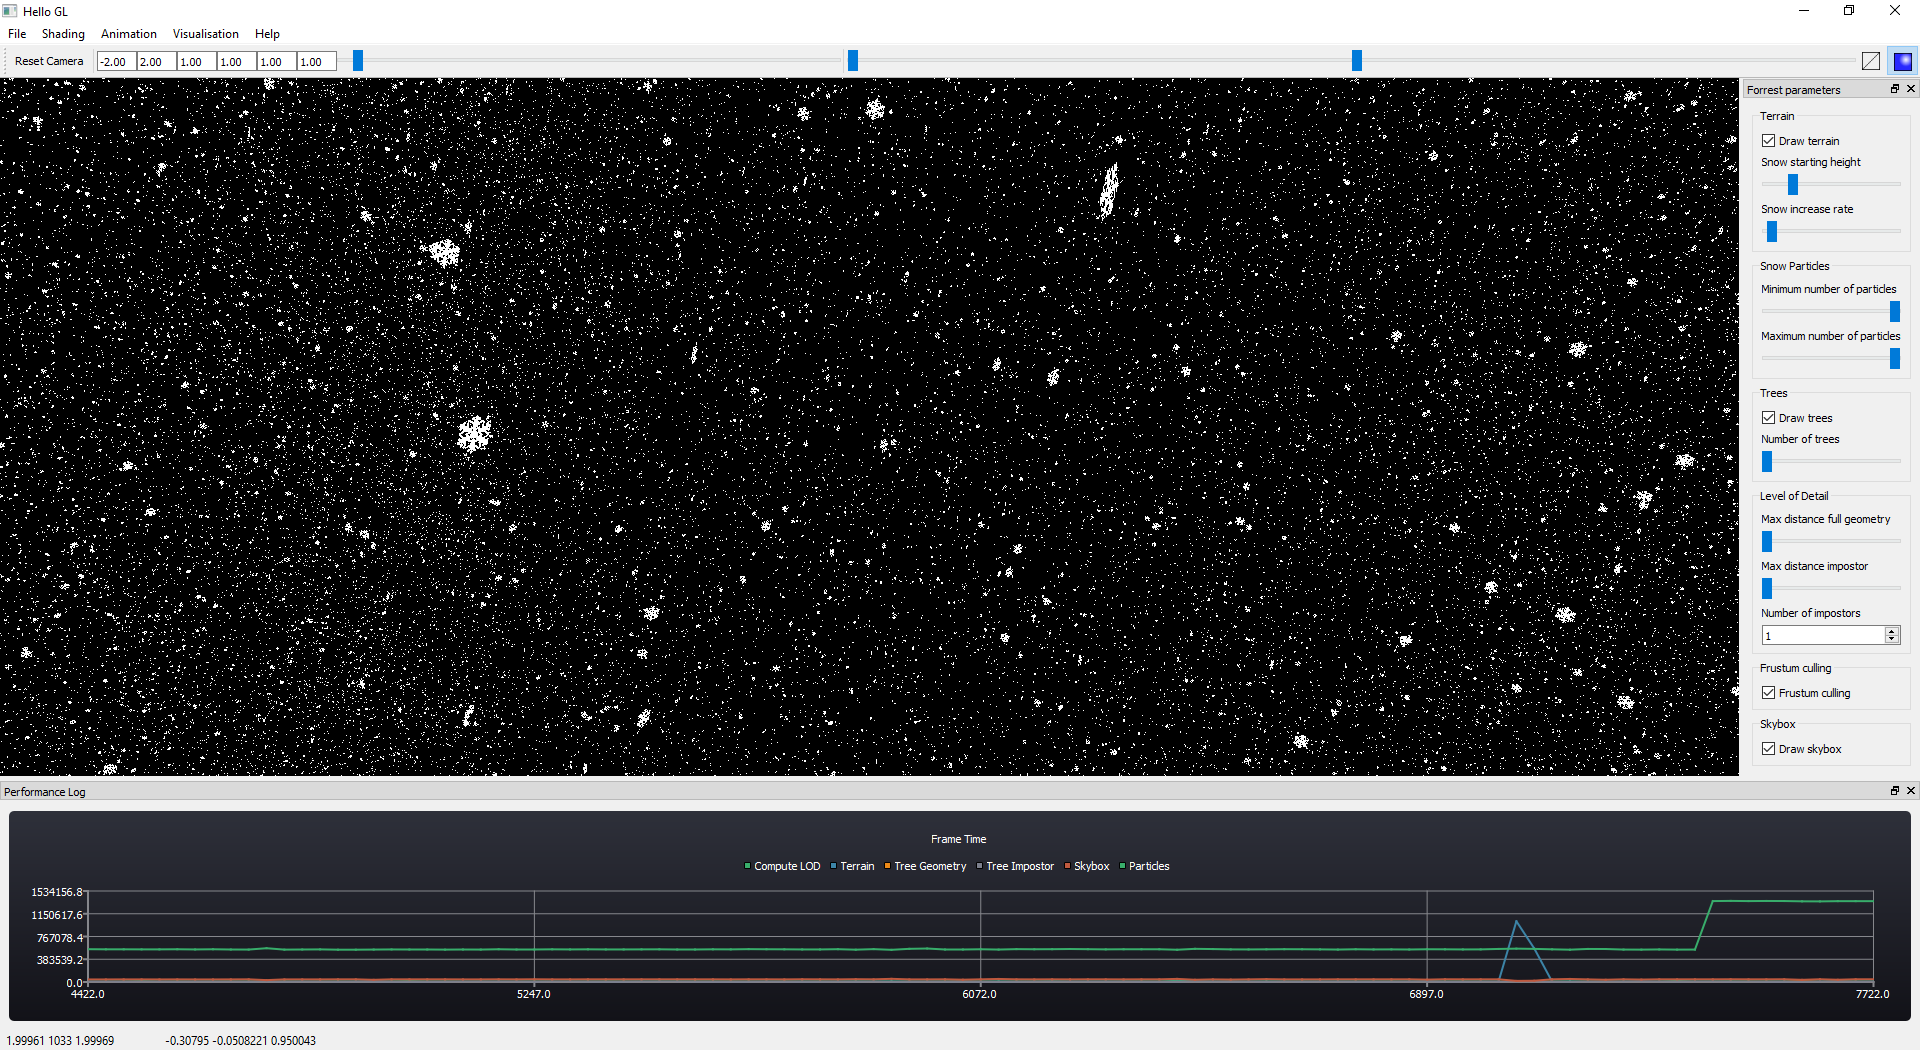
\includegraphics[width=15cm]{images/Particles.PNG}
	\end{figure}
\end{frame}

\begin{frame}{Particle System}
\begin{itemize}
\item Use instanced drawing to draw quads with snowflake texture
\item Create a new buffer for the random particle data (position, rotation)
\item Randomize wind on startup
\item Add a time uniform using QTime
\item In the shader:
\begin{itemize}
	\item Use modulo operation to wrap particles around camera
	\item Animate falling and wind with time uniform
\end{itemize}

\end{itemize}
\end{frame}

\subsection{Volumetric Snow}

\begin{frame}{Terrain - No Snow}
	\begin{figure}[H]
		\centering
		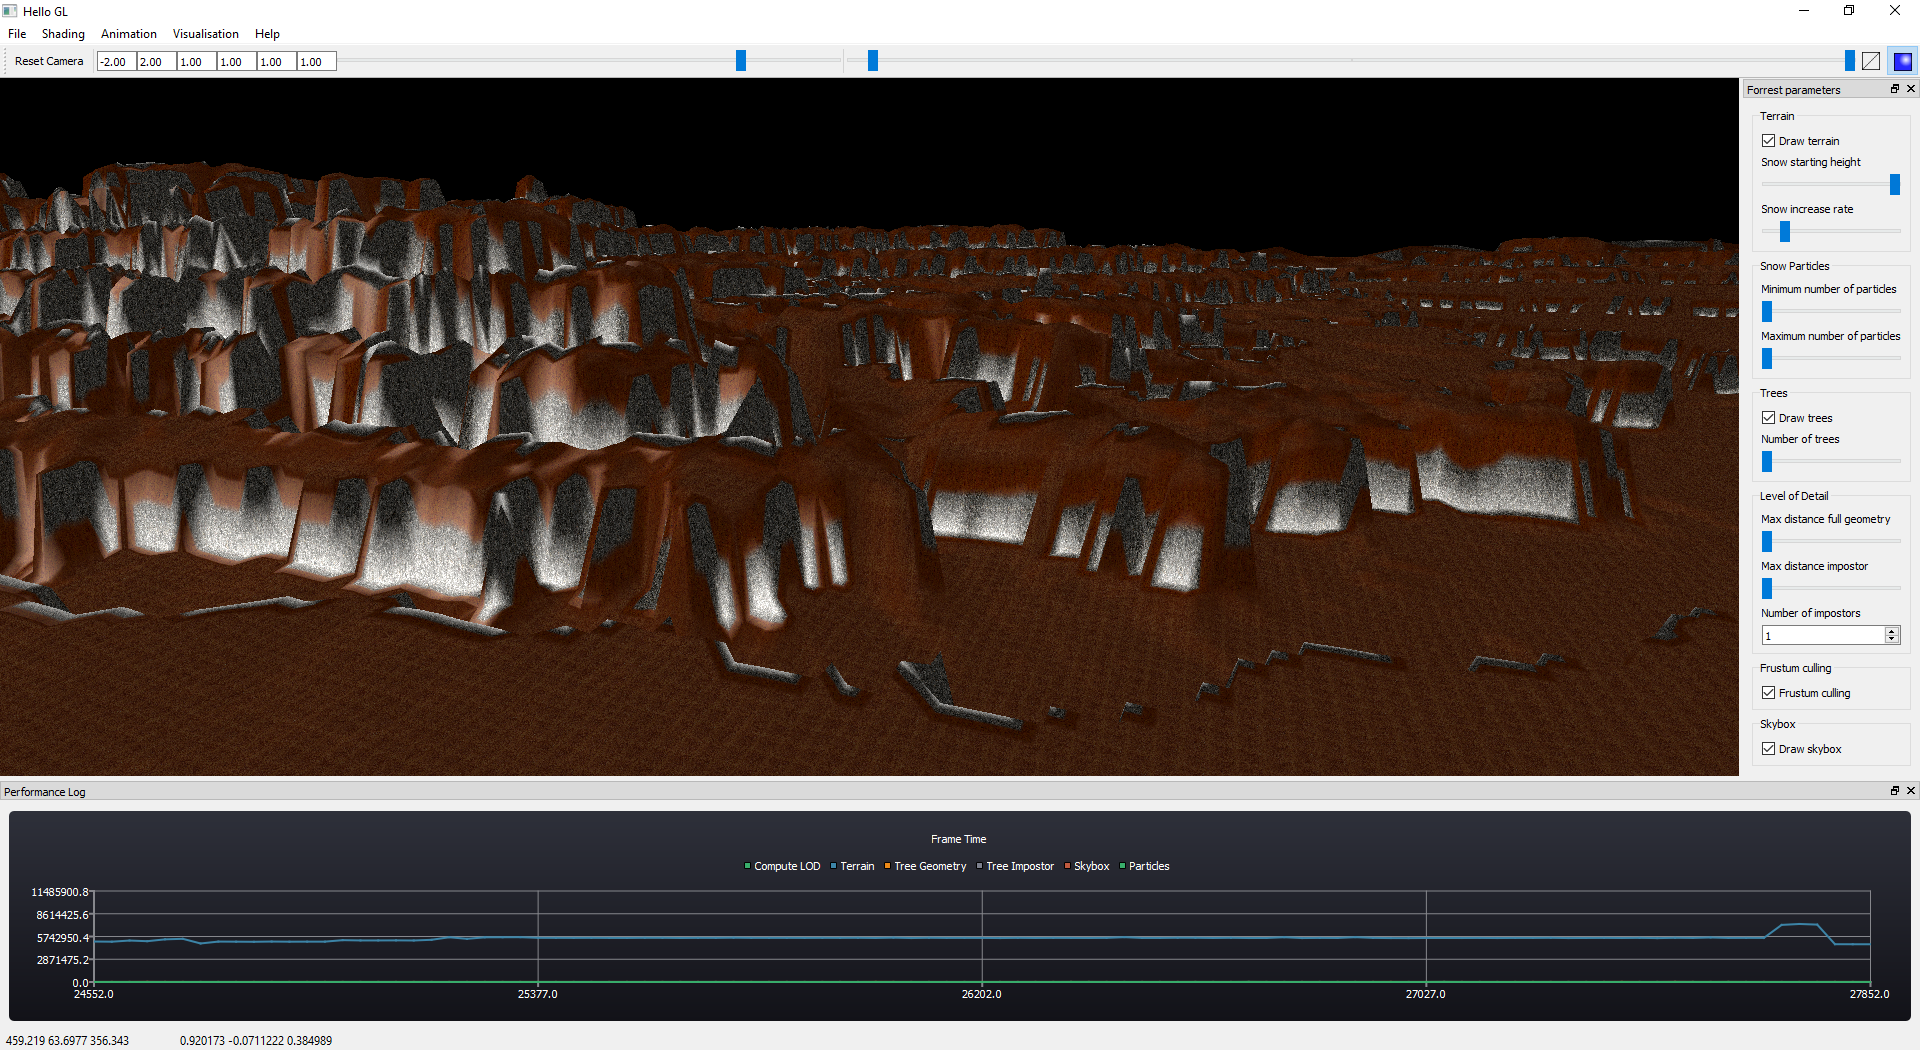
\includegraphics[width=15cm]{images/Terrain-nosnow.PNG}
	\end{figure}
\end{frame}
\begin{frame}{Terrain - Snow}
	\begin{figure}[H]
		\centering
		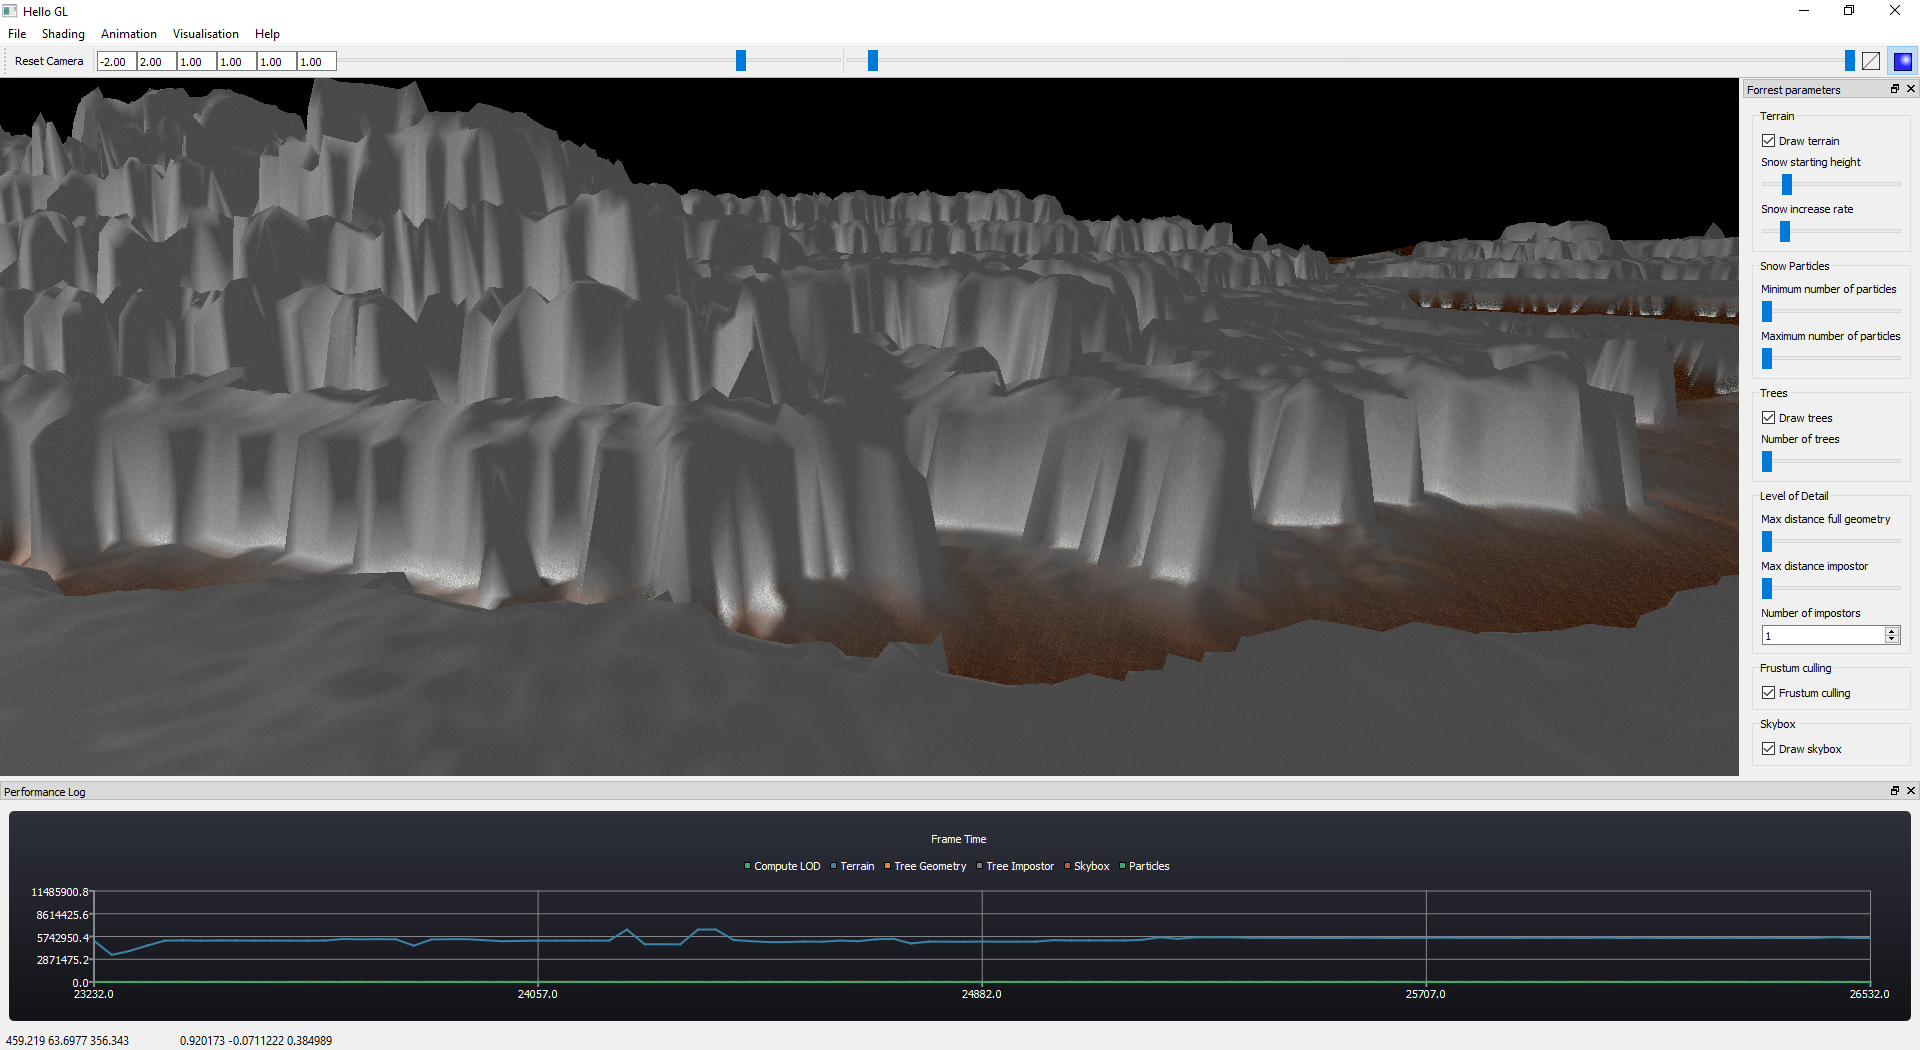
\includegraphics[width=15cm]{images/Terrain-Snow.PNG}
	\end{figure}
\end{frame}

\begin{frame}{Volumetric Snow}
\begin{itemize}
\item Use QImage to store heightmaps
\item Load current snowheight into texture arrays
\item In tessellation evaluation shader:
\begin{itemize}
	\item Access texture array
	\item Move vertex on y-axis
	\item Calculate new normal
\end{itemize}
\item Evaluate lighting equation with new snow texture
\end{itemize}
\end{frame}

\subsection{Refill system}
\begin{frame}{Filling the heightmaps}
\begin{itemize}
\item At startup:
\begin{itemize}
	\item Split terrain into patches
	\item Generate white QImage for each patch
	\item Calculate slope for each pixel of the image
	\item Write slope into alpha channel of the pixel
\end{itemize}
\item Use these images to draw over the current heightmap using a QPainter
\item Load new heightmap into memory
\end{itemize}
\end{frame}

\subsection{Footprints \& snowy trees}
\begin{frame}{Footprints}
	\begin{figure}[H]
		\centering
		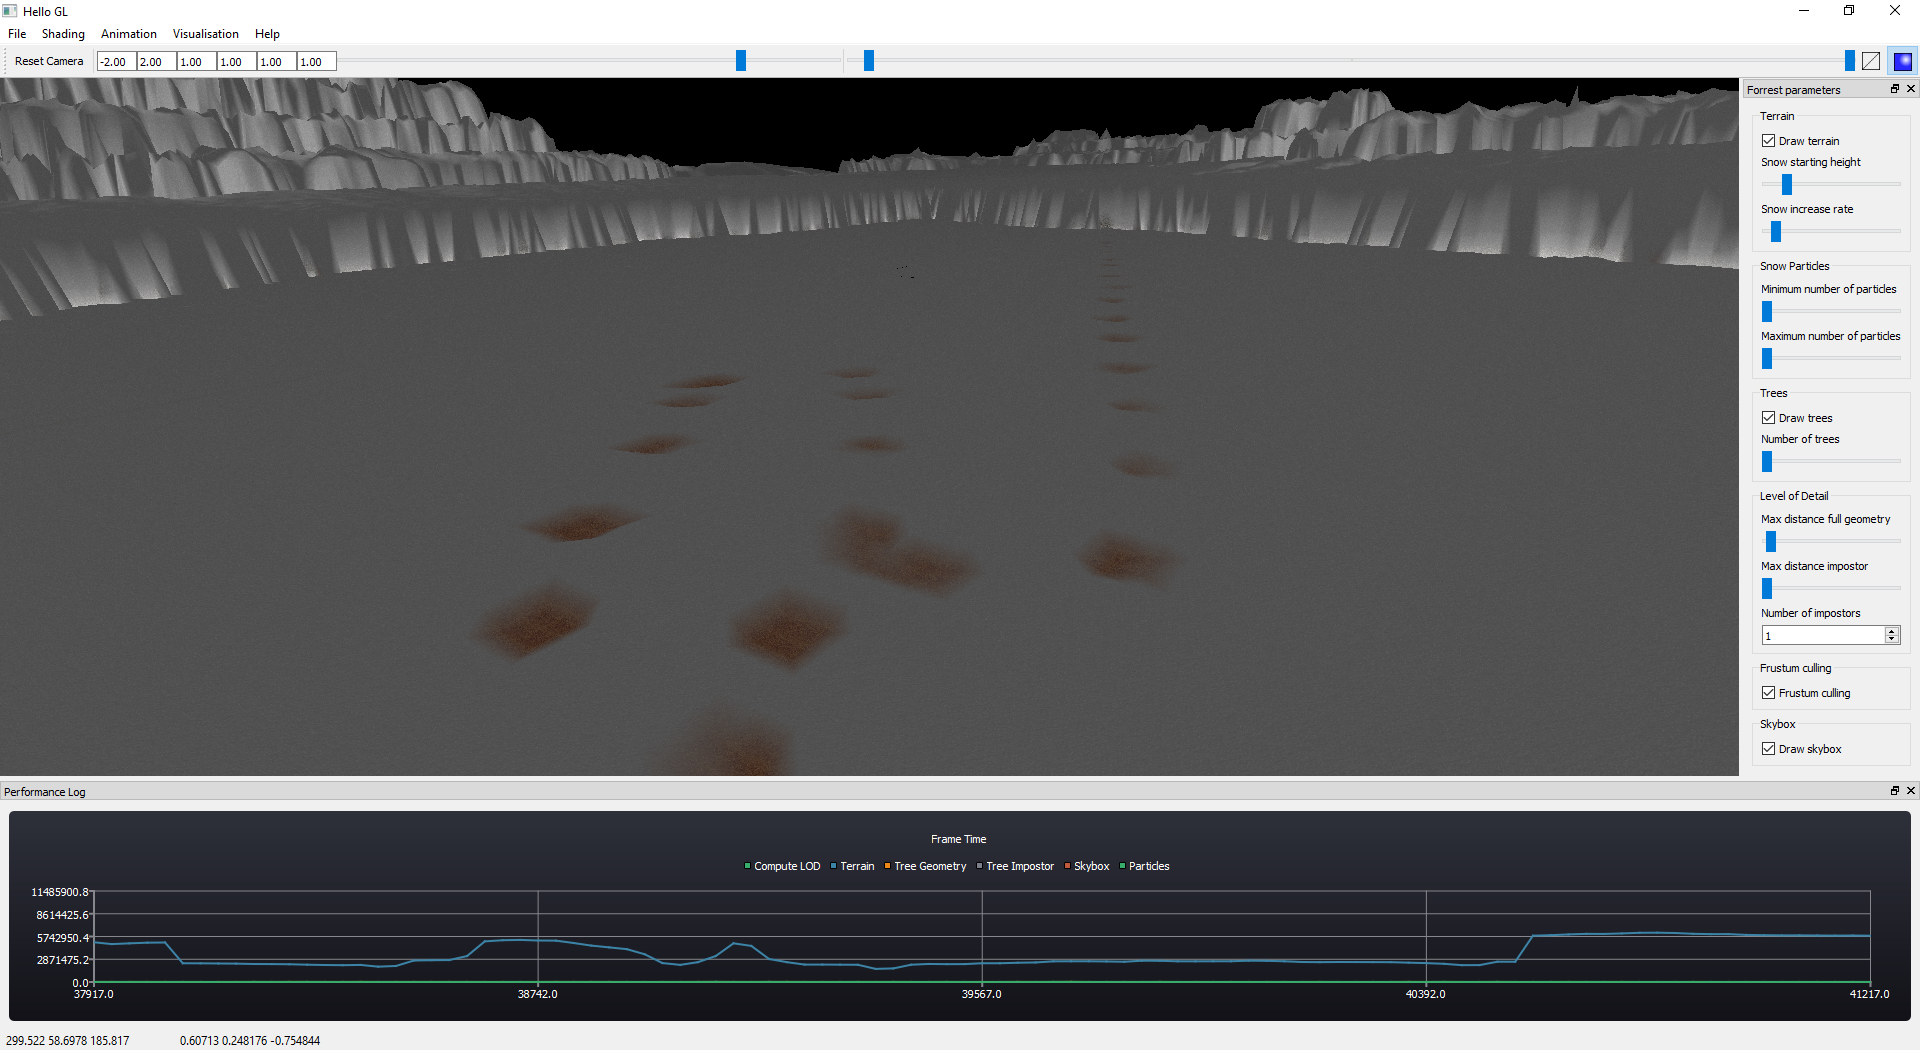
\includegraphics[width=15cm]{images/Footprints.PNG}
	\end{figure}
\end{frame}
\begin{frame}{Snowy Trees}
	\begin{figure}[H]
		\centering
		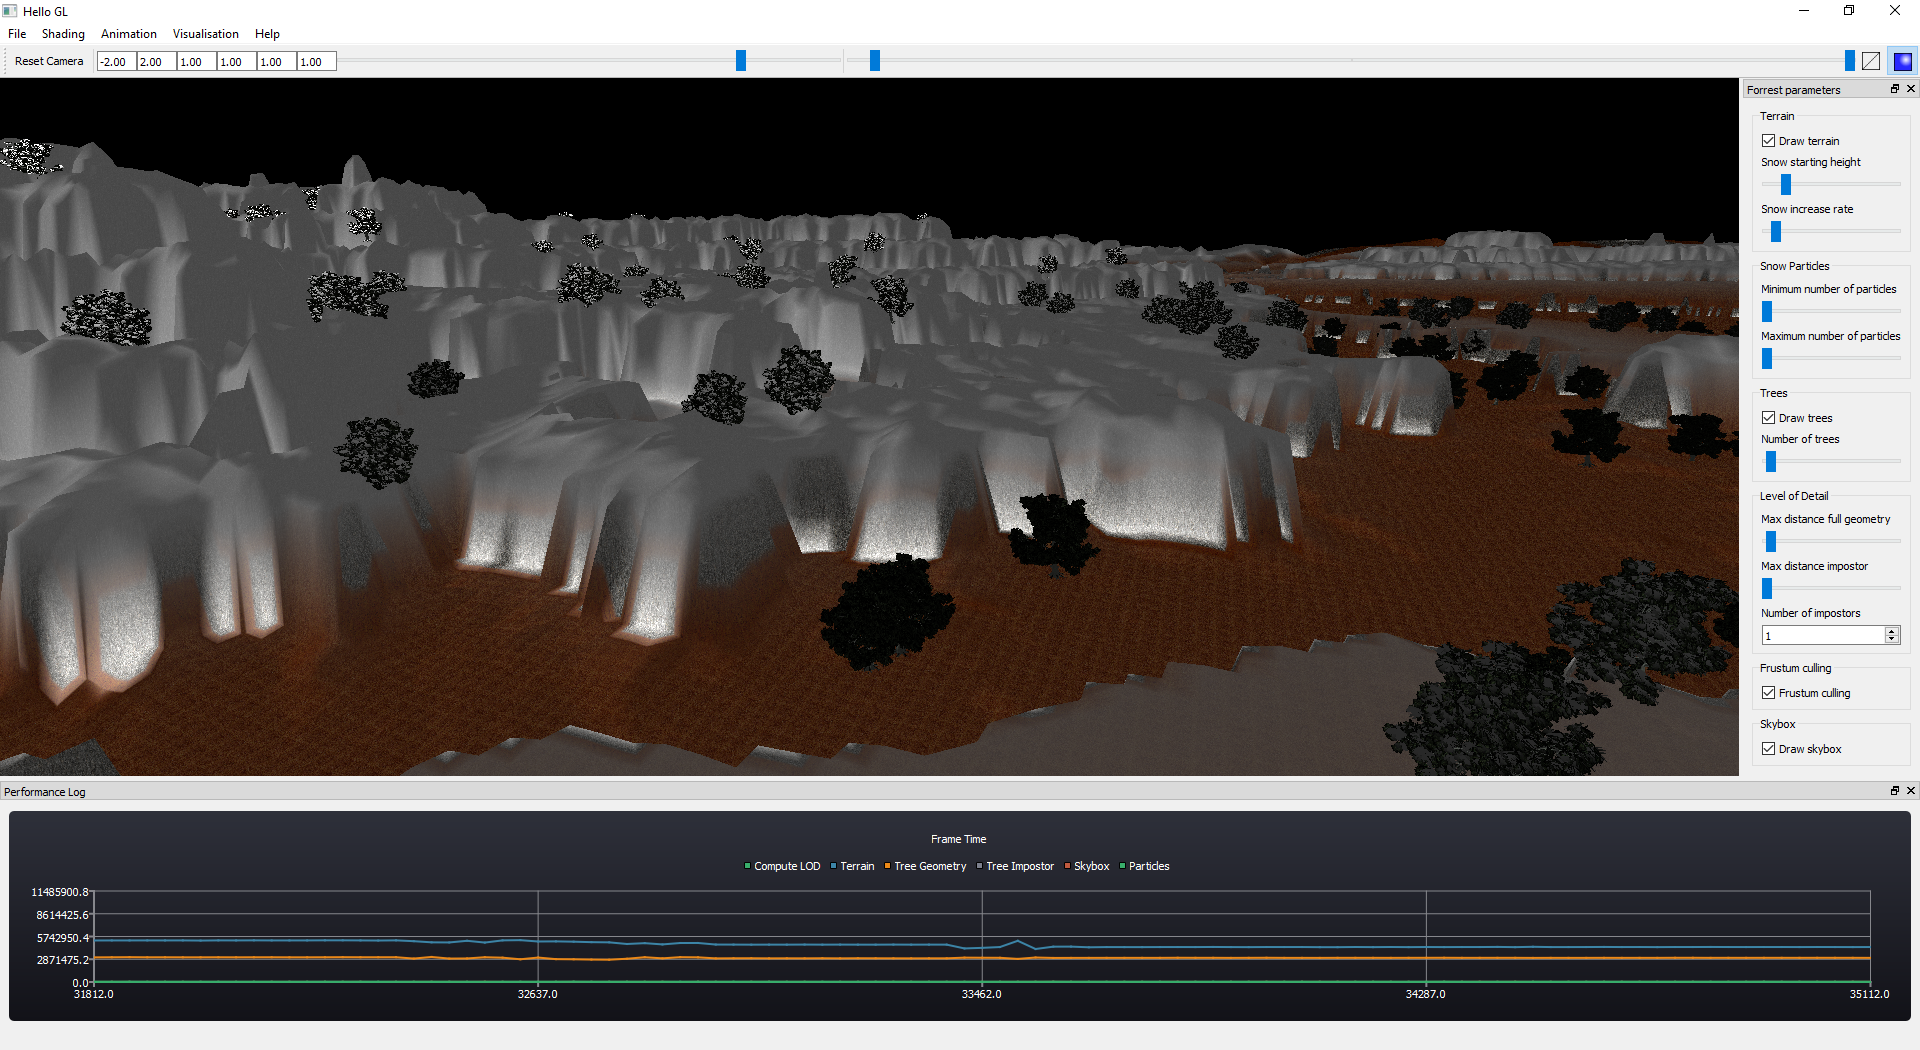
\includegraphics[width=15cm]{images/Trees.PNG}
	\end{figure}
\end{frame}

\begin{frame}{Footprints \& snowy trees}
Footprints:
\begin{itemize}
	\item Use predefined image for a footprint
	\item Determine patch and pixel and draw into heightmap
\end{itemize}
\vspace{0.7cm}
Snowy trees:
\begin{itemize}
	\item Interpolate material with white depending on the normal
	\item Remember alpha testing!
	\item Also use the current height for interpolation
\end{itemize}
\end{frame}

\section{Performance}
\begin{frame}{Performance review}
Main Bottlenecks:
\begin{itemize}
	\item Pixel operations on heightmaps
	\item Slopemap creation
\end{itemize}
\vspace{1.0cm}
The other changes had no severe performance impact!
\end{frame}

\end{document}
